\documentclass[a4paper, top=10mm]{article}
%for writing from the top
\usepackage{fullpage}
%for math
\usepackage{amsmath}
\usepackage{mathrsfs}
\usepackage{amsthm}
\usepackage{amsfonts}
%for images
\usepackage{graphicx}
%for color
\usepackage{xcolor}
%for title
\title{\textbf{\huge{Doctors Numbers}}}
\author{Enigma n\textsuperscript{o}4}
\date{2\textsuperscript{nd} December 2022}

\newtheorem*{hint}{Hint}

\addtolength{\voffset}{-2cm}
\addtolength{\textheight}{5cm}


\begin{document}
	\maketitle
	
	Doctors numbers are special natural numbers such that:
	\begin{itemize}
		\item They start with a "$4$" (in their decimal representation).
		\item When dropping this "$4$", the obtained number is the initial number $N$ divided by $33$\footnote{It is common for French doctors to ask their patients to say "33" (in French) to check their breathing.}.
	\end{itemize}
	
	\vspace{1cm}
	
	\begin{center}
		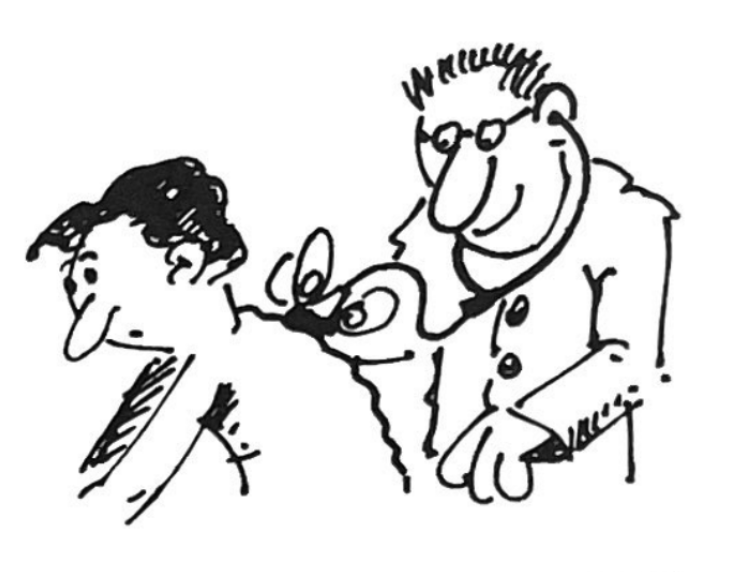
\includegraphics[height=200pt]{04doctor.png}
	\end{center}
	
	\vspace{3cm}
	
	\textbf{What is the smallest doctors number?}
	
\end{document}